\documentclass[sigconf, authorversion=false,  screen=true]{acmart}
\usepackage{color}
\usepackage{booktabs}	% For formal tables
\usepackage{balance}	% to balance the columns on the final page
\usepackage{url}
\usepackage{amsmath}
\usepackage{dirtytalk}

% Copyright
%\setcopyright{none}
%\setcopyright{acmcopyright}
%\setcopyright{acmlicensed}
\setcopyright{rightsretained}
%\setcopyright{usgov}
%\setcopyright{usgovmixed}
%\setcopyright{cagov}
%\setcopyright{cagovmixed}

% DOI
\acmDOI{}

% ISBN
\acmISBN{}

% Prints IU logo in upper left corner
\acmBadgeL{iu}

%Conference
\acmConference[CSCI-B649 IOT]{Internet of Things}
\acmYear{2018}
\copyrightyear{2018}


%\acmArticle{4}
\acmPrice{}

% These commands are optional
%\acmBooktitle{Transactions of the ACM Woodstock conference}
%\editor{Jennifer B. Sartor}
%\editor{Theo D'Hondt}
%\editor{Wolfgang De Meuter}


\begin{document}
\title{A Simple Machine Learning Based Audio Classification Application On ARM Cortex M3}
%\titlenote{Produces the permission block, and copyright information}
%\subtitle{FILL IN SUBTITLE}
%\subtitlenote{The full version of the author's guide is available as
%\texttt{acmart.pdf} document}

\author{Ninaad Joshi}
\affiliation{%
	\position{Graduate Student}
	\department{School of Informatics, Computing, and Engineering}
	\institution{Indiana University}
	\city{Bloomington} 
	\state{Indiana} 
}
\email{ninjoshi@iu.edu}

\author{Rohan Kasture}
\affiliation{%
	\position{Graduate Student}
	\department{School of Informatics, Computing, and Engineering}
	\institution{Indiana University}
	\city{Bloomington} 
	\state{Indiana} 
}
\email{rkasture@iu.edu}

\author{Rohan Shethia}
\affiliation{%
	\position{Graduate Student}
	\department{School of Informatics, Computing, and Engineering}
	\institution{Indiana University}
	\city{Bloomington} 
	\state{Indiana} 
}
\email{rshethia@iu.edu}

\author{Shubham Basu}
\affiliation{%
	\position{Graduate Student}
	\department{School of Informatics, Computing, and Engineering}
	\institution{Indiana University}
	\city{Bloomington} 
	\state{Indiana} 
}
\email{shubasu@iu.edu}

% The default list of authors is too long for headers}
\renewcommand{\shortauthors}{N. Joshi, R. Kasture, R. Shethia, S. Basu}


\begin{abstract}
	\say{\textit{I have not failed. I just found 10,000 ways that won't work.}} --- Nikola Tesla\\
	In this paper we propose an algorithm for automatic detection of a truck sound on a ARM Cortex-M3 processor. The paper talks about the approach taken to achieve audio classification on the Particle Photon along with providing tried and failed alternatives used in the process of coming up with this algorithm. We propose an audio classification method based on decision trees while discussing it’s accuracy compared to the naive bayes classifier. The proposed algorithm is based on two main stages. In first stage, we build the decision tree based on the raw FFT values of truck and non-truck audio samples. In the second stage, we calculate the FFT of the incoming test audio and return the classification result using the decision tree model built. Finally, our experimental results demonstrate that the proposed method is able to achieve an acceptable level of accuracy for classification.
\end{abstract}

%
% The code below was generated by the tool at
% http://dl.acm.org/ccs.cfm
%
\begin{CCSXML}
<ccs2012>
 <concept>
   <concept_id>10002978.10003006.10003007</concept_id>
   <concept_desc>Internet of Things~Machine Learning on Cortex-M3</concept_desc>
   <concept_significance>300</concept_significance>
 </concept>
</ccs2012>
\end{CCSXML}

\ccsdesc[300]{Internet of Things~Machine Learning on Cortex-M3}

\keywords{IOT, Naive Bayes, Decision Trees, ARM Cortex-M3, Digital Signal Processing}

% This turns on page numbering for ACM format and must be before \maketitle
\settopmatter{printfolios=true}

\maketitle

\section{Introduction}
	Trucks produce various sounds when they move, which includes engine noise, body rattling sound, vibrations, horns, etc. But the most dominant noise is from the engine of the truck. The idea of using engine noise to classify trucks seems like a natural choice for a discerning feature. 
	Finding appropriate features is at the heart of an accurate pattern recognition algorithm. There are various features of audio which can be used for classification: temporal features like zero crossing, energy descriptors such short time log energy, noise energy which measure various aspects of signal power and frequency components like cepstral coefficients. But given the limited computational power of the provided hardware, a simple frequency response of the input audio was chosen in order to distinguish between trucks and non-trucks. Since the goal of the on board classification is to just make sure a truck sound is not skipped the choice of frequency response as the deciding feature worked relatively well.
	The paper in the first section provides a brief background on concepts like digital signal processing along with frequency response of a signal and fourier transforms. It also includes machine learning concepts and discusses the difference in approach to making predictions between Naive Bayes and Decision Trees. In the next section the paper goes on to discuss the architecture of the hardware used, that is the ARM Cortex-M3 and the mic mounted on board.The following sections of the paper include the flow diagram and explanation of the experimental setup, results and analysis, future work and conclusion.

\section{Background}

	\begin{figure}
	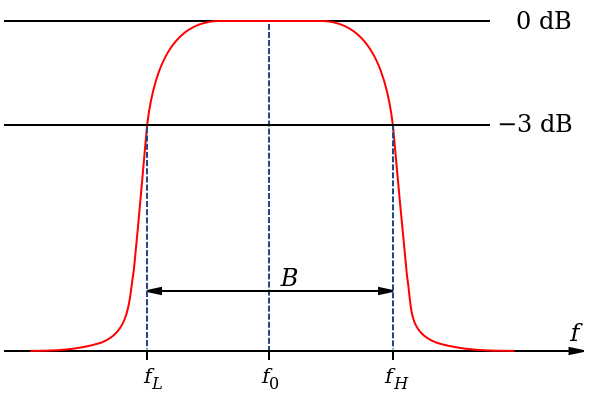
\includegraphics[width=\linewidth]{band_pass}
	\caption{Bandpass filter- Magnitude vs Frequency.~\cite{wiki:bandpass}}
	\label{fig:band_pass}
	\end{figure}
	\subsection{Digital Signal Processing (DSP)}
	Digital signal processing is the technique that takes an already digitized signal (provided by the output of the analog-to-digital converter) and performs various mathematical calculations on the digitized signal. There are various ways to represent the digitized signal, for example: discrete time, discrete frequency, etc so that the signal can be processed further.
	Digital signal processing is used ubiquitously. It is used in applications like, simple graphical representations of signals, audio and video compression, speech processing, speech recognition, digital image processing, and many other applications. Some applications include the implementation of digital filters. As the name suggests, digital filters are used to attenuate or enhance desired portions of the signal.
	Our algorithm uses a digital bandpass filter. In order to fully understand what it does, the paper will discuss a basic model of a digital bandpass filter in this section. A bandpass filter is a circuit (in analog land, and a series of computations in the digital world) whose purpose is to allow signals between two specific frequencies to pass and attenuates rest of the signal. As shown in Figure \ref{fig:band_pass}, signals between f\textsubscript{L} and f\textsubscript{H} are allowed to pass while attenuating the rest of it. Ideally a bandpass filter should completely reject all frequencies out of the passband but it is not so. Frequencies in the vicinity of the limits usually are attenuated and not completely rejected. This is also called roll-off. This is important to note as roll-off turns out to be an important feature that helps us achieve a relatively higher accuracy in our algorithm.
	Another application of DSP is the transform calculation. In DSP, transforms, especially Fourier transforms are used to analyze any signal that varies over time. In this case the signal of interest is an audio signal coming from a truck. The Discrete Fourier Transform (DFT) is used to calculate the signals frequency spectrum. The DFT calculation on a signal results in the decomposition of the signal into its constituent frequencies. We use the Fast Fourier Transform(FFT) calculation which is a standard to calculate the DFT, especially on computers as the asymptotic running time of the simple DFT is O(2n\textsuperscript{2}) where as that of FFT is O(2NlgN)
	
	\subsection{Audio Classification}
	Audio classification is the process of extracting and selecting differentiating features from an audio signal, which is then applied to a trained statistical model (classifier) which then results in the recognition of the audio signal based on the training data. In order to classify audio, researchers have chosen as many as thirty-four features which are claimed as distinguishable. A few of them are; in the frequency domain like Mel Frequency Cepstral Coefficient, spectral centroid, etc which are extracted from the Fourier transform of the signal. In the time domain there are features like short time log energy, which is a log of the energy of the signal for a given window of time.
	\begin{figure}
		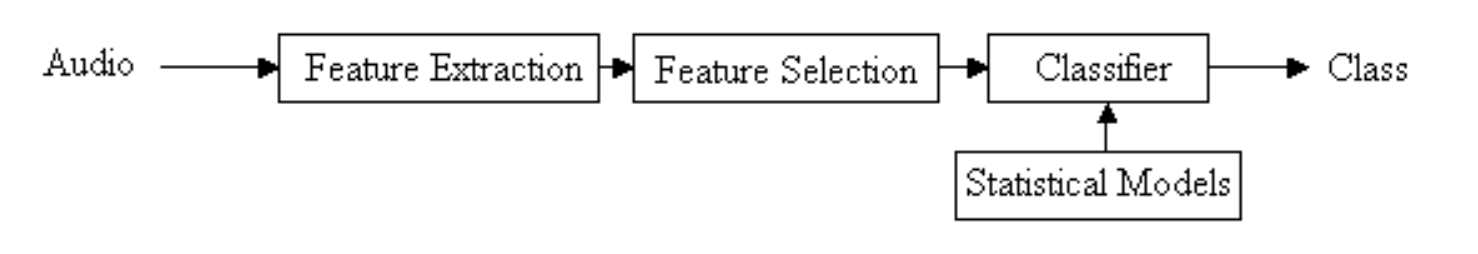
\includegraphics[width=\linewidth]{audio_class}
		\caption{Block diagram for an audio classification system.~\cite{iit:audioclass}}
		\label{fig:audio_class}
	\end{figure}
	
	\subsection{Machine Learning}
	We had two approaches to classify the incoming audio signal as a truck or not. The first approach was to extract the most prominent features from the frequency magnitudes calculated from the audio signal using FFT. For this, we considered the frequencies which would have 70\% or greater magnitude with respect to the maximum magnitude frequency. These features were provided to a Naive Bayes Classifier. Naive Bayes, as the name suggests, is a basic classifier which is not computationally expensive. However, given good differentiating features, Naive Bayes can outperform many other complex classifiers, while being computationally less expensive. The Naive Bayes assumption tells us that the probabilities of any features are independent of each other given the outcome. Given its characteristics, it was considered a good baseline for our project. 
	
	Naive Bayes works by calculating the probability of the sample audio being a truck given the FFT values of the signal. We calculate this probability as follows:
	
	\begin{equation}
	\label{eq:bayes}
	P(Truck|Frequency) = P(Truck) \frac{P(Frequency | Truck)}{P(Frequency)}
	\end{equation}
	
	Where \textbf{P(Frequency)} is:
	
	\begin{equation}
	\begin{aligned}
	\label{eq:bayes2}
	P(Frequency) = P(Frequency | Truck) * P(Truck) +\\ P(Frequency | Non Truck) * P(Non Truck)
	\end{aligned}
	\end{equation}\\
	
	and where \textbf{P(Frequency | Truck)} is as follows:
	
	\begin{equation}
	\begin{aligned}
	\label{eq:bayes3}
	P(Frequency | Truck) = P(Frequency\textsubscript{1} | Truck) *\\ P(Frequency\textsubscript{2} | Truck) *\\ P(Frequency\textsubscript{3} | Truck) *\\ P(Frequency\textsubscript{n} | Truck)
	\end{aligned}
	\end{equation}\\
	
	Where ‘n’ is the number of frequencies we consider. (n = 1024 buckets in our case. Which is the entire spectrum from 1Hz to 44.1KHz)
	
	While Naive Bayes was less expensive in terms of computation, we found that the classification accuracy was not good enough for our needs and we could only achieve a meager accuracy of 45-50\%. Thus, we decided to use a different but more robust classifier called the Decision Tree.
	
	\begin{figure*}
		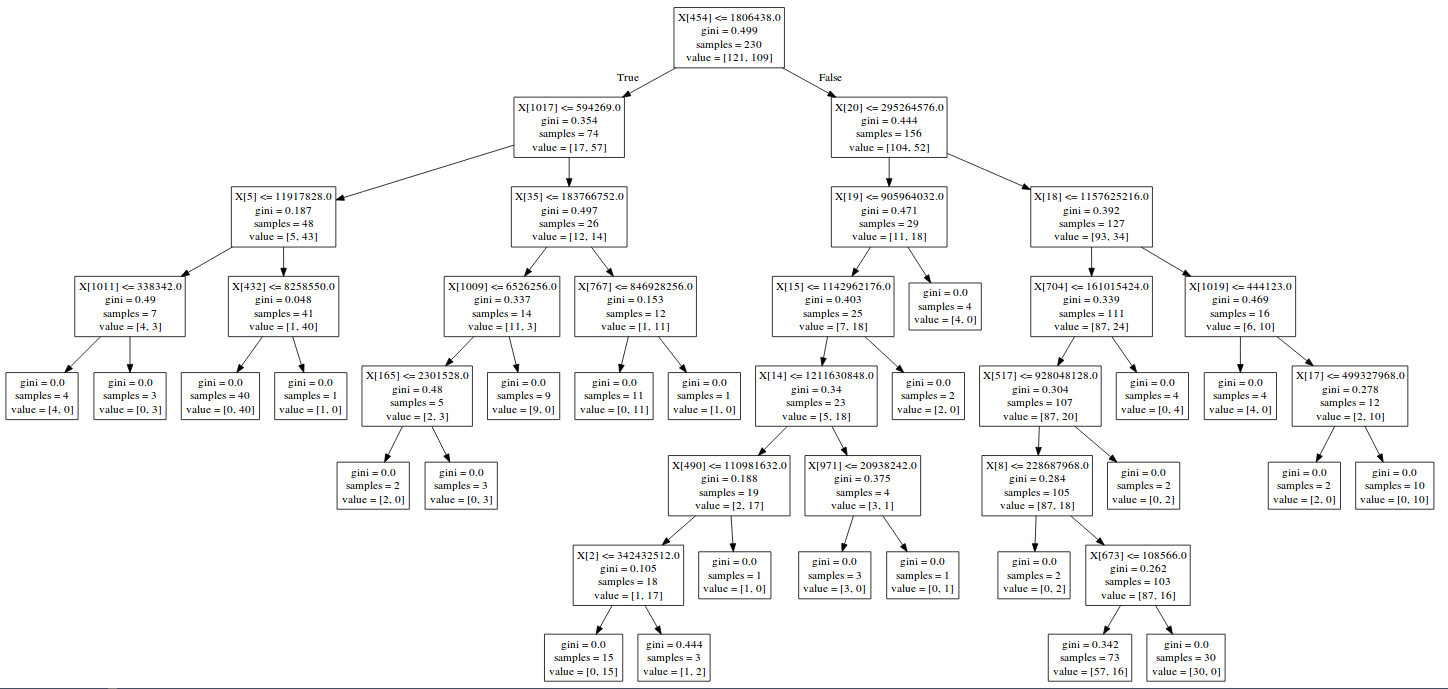
\includegraphics[width=\linewidth]{decision_tree}
		\caption{The decision tree generated for our algorithm. The gini value i.e. percentage of the split at each node of the decision tree determines the weight of the decision using the conditional statements. The number of samples at each node indicate the samples which abide by the decision. }
		\label{fig:dec_tree}
	\end{figure*}

	The Decision Tree classifier can be considered as a sequence of nested condition statements, which consider the different features, in our case the FFT values, in order to  generate a decision.
	
	The Decision Tree was able to give better results compared to the Naive Bayes Classifier, as we were able to achieve an accuracy in the range of 69-75\%. Thus, we decided to move forward with the Decision Tree classifier.
	
	We first implemented the decision tree in Python using the FFT values generated on the Photon. We used the ‘Scikit-Learn’\cite{sklearn_api} library for the implementation. We generally provide a maximum depth while creating a decision tree to avoid over-fitting of the data points. Each node generates a decision for a particular frequency. We decided not to provide a maximum depth for the tree. This was based on the fact that using a bandpass filter had reduced the vast number of frequency points over which decision conditions would have to be made, thereby limiting the depth of the tree naturally.
	The percentage of the split at each node of the decision tree determines the weight of the decision using the conditional statements. After the decision tree was generated, we converted our implementation to C code for the Photon and integrated the decision tree in the Photon.
	
\section{Experiment Setup}
	
	\subsection{Hardware  Components}
	The hardware we use for this project is the Particle Photon, which is an embedded board that hosts STM's implementation of ARM's Cortex-M3 processor along with other components. It is a 32-bit processor that runs at 120MHz. It is important to note that this processor lacks a Floating Point Unit (FPU). While this is advantageous for low power consumption, it limits the capabilities of what the board can do. The board comes with 128KB of RAM and 1MB of flash to hold the firmware. Another important component of this system is the Broadcom BCM43362 Wi-Fi chip. The initial power consumption measurements indicate that this is the most power hungry component on this board. We use one out-of-board component in our set up and that's the ADMP401 microphone. It is a low power, MicroElectrical-Mechanical System (MEMS) mic, with a high signal to noise ratio (SNR). It is interesting to note that this microphone has a gain of 67.

	\subsection{The Setup}
	\begin{figure}
		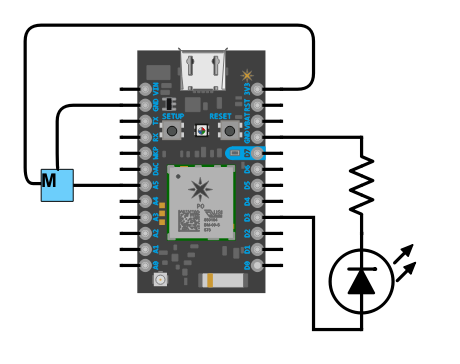
\includegraphics[width=\linewidth]{photon}
		\caption{Circuit diagram of the Photon setup. The microphone (M) provides analog input to A5 and the LED is connected to D3.}
		\label{fig:photon}
	\end{figure}

	Our setup includes the microphone connected to the Particle Photon and a white LED indicator which glows when a positive response from the server running the advanced classifier is received. The FFT values were generated on the photon. These values were used to generate a decision tree using the SciKit Learn Library. Note: The decision trees depth was not limited. The generated model was then converted to C code and implemented on the photon as a function which returned a value for truck or no-truck based on the FFT generated at run time for the incoming signal. 
	During testing, in order to avoid false positives the photon would transmit the audio signal to the cloud only if it classified the incoming audio as truck thrice. After getting three consecutive positive decisions from the classifier model, the WiFi is enabled (note that WiFi is disabled for all times other than transmission of the audio data in order to conserve energy) and the audio signal is transmitted to the cloud where in an ideal scenario an advanced classifier like a neural net is running. Once the server classifies it as a truck it will send back a response to the photon. If the cloud response is positive, the white LED glows for one second, thus, indicating that the audio signal has been successfully determined to be originated from a truck.
	An important aspect of our model building was that we trained our classifier on the entire frequency spectrum of 44100Hz (i.e. buffer size of 1024). This is where roll-off helped improve our classification accuracy. Simply ignoring frequencies over 800Hz made no sense as those frequencies, no matter what magnitude still lend weight while training the decision tree.	
	
	\begin{figure}
		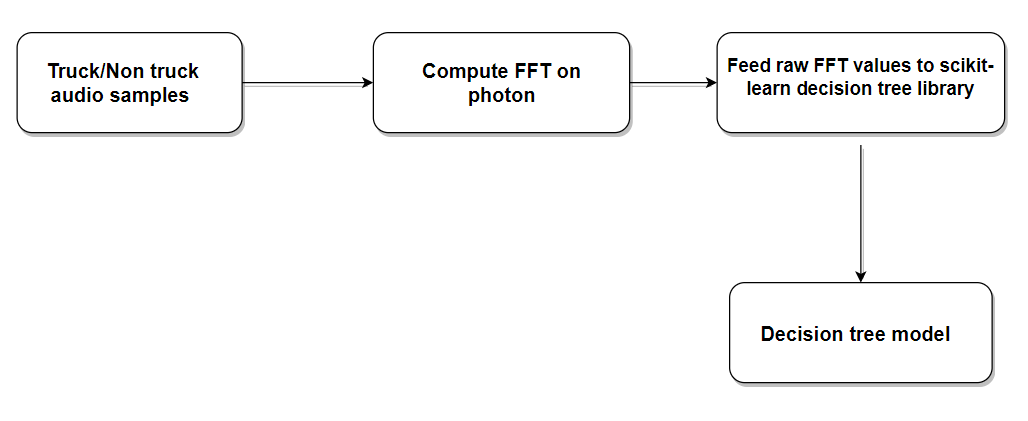
\includegraphics[width=\linewidth]{1}
		\caption{Flow diagram for building the decision tree model for classification.}
		\label{fig:1}
	\end{figure}

	Figure \ref{fig:1} describes the first half of our algorithm. First a few hundred samples of Trucks and Non-Trucks audio are fed into the Photon via the microphone after which the FFT is locally computed and the FFT values are streamed out to the server. The computed FFT values are given to the Sci-Kit Learn Library which outputs the decision tree model shown in Figure \ref{fig:dec_tree}.
	
	\begin{figure}
		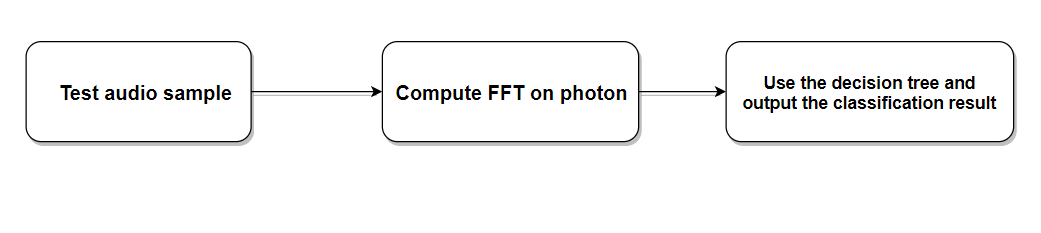
\includegraphics[width=\linewidth]{2}
		\caption{Flow diagram for building the decision tree model for classification.}
		\label{fig:2}
	\end{figure}

	Figure \ref{fig:2} describes the second half or validation part of our algorithm. The test audio is provided to the Photon after which the FFT is computed and fed into the model which provides a classification in real time.
    
\section{Trials and Evaluation}
	Our first objective for the classification of truck audio signals was to use a simple classifier on the Particle Photon which would be able to distinguish between truck and non truck sounds. The main reason behind detecting non truck audio was to save as much power on the transmission of audio to the cloud as possible. The Photon drew the most power during the transmission of audio to the cloud using WiFi. Thus, we had to make sure that the Photon would transmit the audio only if it was a genuine truck audio signal.

	\begin{figure}
		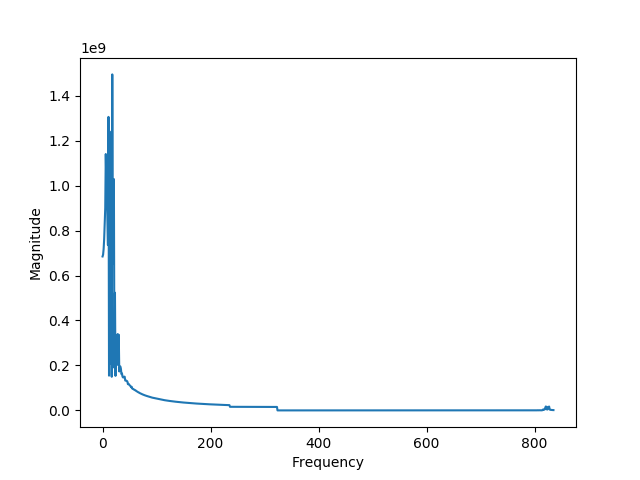
\includegraphics[width=\linewidth]{truck_after_filter}
		\caption{Fast Fourier Transform Plot of Truck audio after passing through a bandpass filter}
		\label{fig:truck_after_filter}
	\end{figure}
	
	Figure \ref{fig:truck_after_filter} shows a plot of the frequency response of the truck audio after filtering. It is clearly visible that the range of 200Hz to 800Hz is dominating.
	
	\begin{figure}
		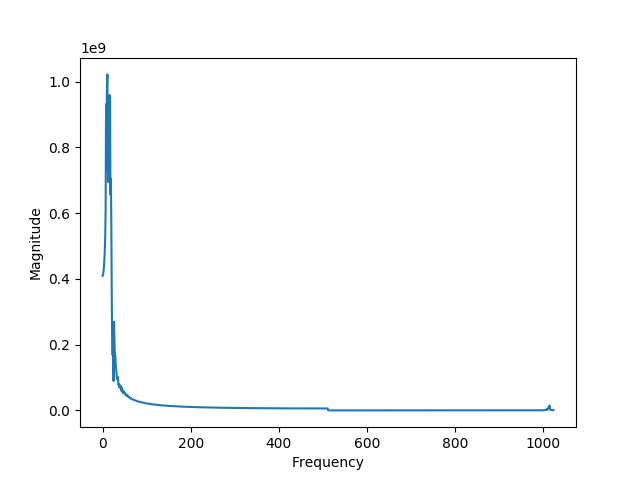
\includegraphics[width=\linewidth]{no_truck_after_filter}
		\caption{Fast Fourier Transform Plot of Non-Truck audio after passing through a bandpass filter}
		\label{fig:no_truck_after_filter}
	\end{figure}

	Figure \ref{fig:no_truck_after_filter} shows a plot of the frequency response of the non-truck audio after filtering. The region of from 200Hz to 800Hz is sparse and this is where we get our dominating feature for classification. It is interesting to note the difference in roll-off as well. Usually roll-off is an undesirable characteristic of filters but in this case the difference in roll-off improves the weight of classification. Another noticeable observation is that non-truck sounds have an attenuated signal in the 1000Hz region while there is almost no signal after 800Hz for trucks, as seen in Figure \ref{fig:truck_after_filter}. This was another reason why considering the entire buffer of 1024 (containing all 44100Hz) for decision making turned out to make our model relatively more accurate.

	We tried a few techniques for truck audio classification which provided results that were not as  promising as the one with decision tree model. We started with off building a simple Naive Bayes classifier in python which would classify the input test audio into either of the two classes namely truck or non truck based on the probability values. The size of the physical memory of Photon micro-controller puts a limit on number of samples of FFT that can be used for audio classification. We tried with various length of FFT values i.e 24,100,1024,etc. The downside to using lesser FFT samples results in the loss of resolution. When you use 24-size FFT buffer you bucket 43 frequency values in every bucket and the maximum frequency represented by this FFT buffer would be 1033Hz. This bucketing of frequencies leads to inaccurate classification results as Naive Bayes does not do very well with low resolution data.  

	Another feature based on which we tried to classify is the zero crossing rate of a filtered signal. The zero-crossing rate is the rate of sign-changes along a signal, i.e, the rate at which the signal changes from positive to negative or back. Zero crossing normally occurs twice during each cycle in a sine wave. We calculated the zero-crossing rate for both truck and non-truck audio samples but there was no discernible change in the rate of zero-crossing for trucks and non trucks. Not being able to clearly differentiate truck from non-truck samples with zero-crossing rate, led us to discarding this approach.
	
	\begin{figure}
		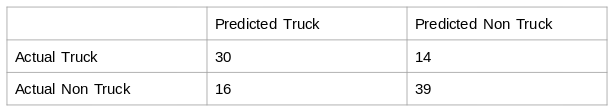
\includegraphics[width=\linewidth]{confusion}
		\caption{Decision Tree Confusion Matrix: Total Samples: 99. True Positives: 30. True Negatives: 39. False Positives: 16. False Negatives: 14}
		\label{fig:confusion}
	\end{figure}
	
	After going through multiple approaches, decision trees seemed to give us the most reliable results. The confusion matrix is shown in Figure \ref{fig:confusion}. The confusion matrix is an evaluation of a classifier model. It displays a count of true positives, true negatives, false positives and false negatives. Ideally one would want to have zero false positives and false negatives, hence this becomes a benchmark against which the performance of a classifier can be evaluated. Our primary aim was to minimize the number of false negatives, that is classification of truck as non-truck along with achieving an acceptable level of false positives. As one can see from Figure \ref{fig:confusion}, the rate of false negatives is at a decent 14.14\% while the rate of false positives is at an acceptable 16.16\%.
	
\section{Future Work and Conclusion}
	We developed a decision tree based classification strategy to solve the truck audio classification problem. We achieved an accuracy of ~70\% with the decision tree based model. This opens up the possibility for future research in a various directions. Different types of classifiers can be used for classification. For example, we could use a Neural Net to find the valuable features and their weight accordingly. We could then use the generated model on the Photon to classify the audio with higher accuracy. We can make use of other audio features like cepstral coefficients, etc. rather than just using raw FFT values for audio classification. This would be helpful in greatly enhancing the accuracy of the current implementation. 
	Another primary aspect of this study would be to address the power efficiency measurements. A few of the many states in which measuring the power consumption of the photon would provide an insight into the efficiency of the application could be, while just in standby mode, while listening to incoming audio and computing FFT in real time, while streaming out audio samples over a TCP connection to the cloud.
	One potential application of our project would be to detect potential lawbreakers who violate traffic rules by not using specific lanes meant for trucks or other heavy vehicles. Another possible application of an audio sensor node like this could be for espionage as well. The key objective for these applications or any other application would be, to try and keep the power consumption as low as possible so that the nodes do not have to be replaced often.
	
\bibliographystyle{ACM-Reference-Format}
\bibliography{report} 

\balance
\end{document}
